%%%%%%%%%%%%%%%%%%%%%%%%%%%%%%%%%%%%%%%%%%%%%%%%%%%%%%%%%%%%%%%%%%
%%%%%%%% ICML 2012 EXAMPLE LATEX SUBMISSION FILE %%%%%%%%%%%%%%%%%
%%%%%%%%%%%%%%%%%%%%%%%%%%%%%%%%%%%%%%%%%%%%%%%%%%%%%%%%%%%%%%%%%%

% Use the following line _only_ if you're still using LaTeX 2.09.
%\documentstyle[icml2012,epsf,natbib]{article}
% If you rely on Latex2e packages, like most moden people use this:
\documentclass{article}

% For figures
\usepackage{graphicx} % more modern
%\usepackage{epsfig} % less modern
\usepackage{subfigure} 

% For citations
%\usepackage{chicago}
\usepackage{natbib}



% For algorithms
\usepackage{algorithm}
\usepackage{algorithmic}
\usepackage{amsmath}
\usepackage{amsfonts}
\usepackage{amsthm}
\newtheorem{theorem}{Theorem}
\newtheorem{lemma}[theorem]{Lemma}
\usepackage{amsmath}               
  {
      \theoremstyle{plain}
      \newtheorem{assumption}{Assumption}
      \theoremstyle{definition}
      \newtheorem{modification}{Moditication}
  }

% As of 2011, we use the hyperref package to produce hyperlinks in the
% resulting PDF.  If this breaks your system, please commend out the
% following usepackage line and replace \usepackage{icml2012} with
% \usepackage[nohyperref]{icml2012} above.
\usepackage{hyperref}

% Packages hyperref and algorithmic misbehave sometimes.  We can fix
% this with the following command.
\newcommand{\theHalgorithm}{\arabic{algorithm}}

% Employ the following version of the ``usepackage'' statement for
% submitting the draft version of the paper for review.  This will set
% the note in the first column to ``Under review.  Do not distribute.''
\usepackage[accepted]{icml2012} 
% Employ this version of the ``usepackage'' statement after the paper has
% been accepted, when creating the final version.  This will set the
% note in the first column to ``Appearing in''
% \usepackage[accepted]{icml2012}


% The \icmltitle you define below is probably too long as a header.
% Therefore, a short form for the running title is supplied here:
\icmltitlerunning{Submission and Formatting Instructions for ICML 2012}

\begin{document} 
\twocolumn[
\icmltitle{CS 6780 Research Project: Multi-armed Bandits with Dependent Arms}

% It is OKAY to include author information, even for blind
% submissions: the style file will automatically remove it for you
% unless you've provided the [accepted] option to the icml2015
% package.
\icmlauthor{Bangrui Chen}{bc496@cornell.edu}
\icmlauthor{Saul Toscano Palmerin}{st684@cornell.edu}
\icmlauthor{Zhengdi Shen}{zs267@cornell.edu}

% You may provide any keywords that you 
% find helpful for describing your paper; these are used to populate 
% the "keywords" metadata in the PDF but will not be shown in the document
\icmlkeywords{boring formatting information, machine learning, ICML}

\vskip 0.3in
]

\begin{abstract} 
We study the multi-armed bandits problem where the reward of each arm  depends linearly on a multi-variate random variable. We provide three heuristic algorithms based on the PEGE algorithm \cite{Paat}. We prove that our first heuristic algorithm still has Bayes risk $O(r\sqrt{T})$. Numerical experiments suggest that our new algorithms outperform the PEGE algorithm as well as the Exponential Gradient algorithm. 
\end{abstract} 


\section{Introduction}

Exploration vs. Exploitation has been studied extensively under the framework of multi-armed bandits problem. The multi-armed bandits (MAB) problem was first studied by Robbins \cite{Robbins}. The goal of MAB is to find the optimal policy so that we can pull arms sequentially in order to maximize the total expected reward. For the case where each arm is independent, the Gittins Index \cite{Gittins} provides an optimal policy for maximizing the expected reward. Further, Lai and Robbins \cite{Lai} prove that the regret under an arbitrary policy increases linearly with the number of arms. Most policies that assume independence require each arm to be tried at least once, which are impractical in settings involving many or infinite arms. 

Since then, a lot of research has been focused on the dependent case. In \citet{Gabor} and \citet{Chih-Chun}, the multi-bandit problem with side information is studied. In \citet{Yasin1,Yasin2} , the reward for each bandit is the inner product between a single unknown parameter and the bandit. In \citet{Paat}, the expected reward of each arm depends linearly on a multivariate random variable. Furthermore, it is showed that under an arbitrary policy, the Bayes risk is at least $O(r\sqrt{T})$ where r is the dimension of the multivariate random variable. The authors also provide a simple Phased Exploration Greedy Exploitation (PEGE) algorithm that reaches the $O(r\sqrt{T})$ Bayes risk bound.

Though PEGE reaches the optimal Bayes risk bound, it does not perform well in practice. In this project, we modify the PEGE algorithm and get three heuristic algorithms. We prove that the first modified algorithm is still optimal in the sense that its Bayes risk is still $O(r\sqrt{T})$. We perform numerical experiments using the Yelp academic data to compare our modified algorithms as well as the original PEGE algorithm. The results suggest that our modified algorithms are much better. Further, we compare our modified algorithms with UCB and Exponential Gradient algorithm (EXP). Although UCB algorithm outperforms our new algorithms in the experiments, it requires previous knowledge about the multivariate random variable, which is impossible for the ``cold start" problems. Our heuristic algorithms perform better than EXP and PEGE, and do not require any previous information.

There are lots of applications of this problem. For example, given a fixed budget, the problem is to allocate resources among competing projects, whose properties are only partially known at the time of allocation, but which may become better understood as time passes. MAB is also closely related to the recommender systems, which are a subclass of information filtering system that seek to predict the ``rating" or ``preference" that user would give to an item. For instance, how should a electronic commerce company like Amazon select forwarding items to a newly registered user? In these applications, one natural question would be how can we quickly learn projects' properties or user's preference from their feedback? All of these problems can be modeled as a multi-armed bandit problem and our heuristic policies can be applied.





\section{Problem Formulation}
We have a finite set $\mathcal{U}_{r}=\{\bold{u}_{1},\cdots,\bold{u}_{m}\}\subset \mathbb{R}^{r}$ (or infinite set $\mathcal{U}_{r}=\{\bold{u}_{1},\cdots,\bold{u}_{m},\cdots\}\subset \mathbb{R}^{r}$) that corresponds to the set of arms, where $r\geq 2$. For any time $t=1,2,\cdots,T$, we are asked to pick one arm $X_{t}$. The reward $Y_{t}$ of playing arm $X_{t}\in \mathcal{U}_{r}$ in period t is given by
\begin{equation}
Y_{t} = \theta \cdot X_{t} + \epsilon_{t}, \nonumber
\end{equation}
where $\epsilon_{t}\sim N(0,\sigma^{2})$ is the measurement error with $\sigma$ known and remains the same overtime. Here $\theta$ is an unknown random vector. When implementing UCB algorithm, we require $\theta$ is drawn from a multivariate normal distribution with mean $\mu$ and variance $\Sigma$. We further assume $\mu$ and $\Sigma$ are known when. 

For a fixed time period T, the goal of this problem is to find a strategy $\pi$ to maximize the following expression
\begin{equation}
E^{\pi}\left[\sum_{t=1}^{T} Y_{t}\right].
\end{equation}
Or equivalently, we are trying to find a policy that can minimize the Bayes risk under $\pi$:
\begin{equation}
\text{Risk}(T,\pi) = E\left[\text{Regret}(\theta,T,\pi)\right],
\end{equation}

where the cumulative regret is defined as the following:
\begin{equation}
\text{Regret}(\theta_{0},T,\pi)=\sum_{t=1}^{T}E\left[\max_{X\in \mathcal{U}_{r}}X\cdot\theta_{0}-X_{t}\cdot \theta_{0}|\theta=\theta_{0}\right].
\end{equation}





\section{PEGE}

Theoretically this problem can be solved using stochastic dynamic programming, such as backward induction. However it usually suffers from the curse of dimensionality when the dimension of the arm, i.e. r is large. Thus, it is desirable to develop some computational feasible heuristic algorithms.

In \citet{Paat}, they prove the following theorem which gives a lower bound for the Bayes risk:

\begin{theorem}(Lower Bound)
Consider a bandit problem where the set of arms is the unit sphere in $\mathbb{R}^{r}$, and $\epsilon_{t}$ has a standard normal distribution with mean 0 and variance one for all t and $X_{t}$. If $\theta$ has a multivariate normal distribution with mean $\bold{0}$ and covariance matrix $\bold{I}_{r}/r$, then for all policies $\pi$ and every $T\geq r^{2}$,
\begin{equation}
\text{Risk}(T,\pi)\geq 0.006r\sqrt{T}. \nonumber 
\end{equation}
\end{theorem}

In their paper, they also provide a simple algorithm called Phased Exploration and Greedy Exploitation (PEGE) (Algorithm 1) that reaches the corresponding lower bound, i.e the Bayes risk for PEGE is $O(r\sqrt{T})$. In order for the algorithm to work, it requires the following two assumptions:

\begin{assumption}
\begin{itemize}
\item There exists a positive constant $\sigma_{0}$ such that for any $r\geq 2$, $\textbf{u}\in \mathcal{U}_{r}$, $t\geq 1$ and $x\in \mathbb{R}$, we have $E[e^{x \epsilon_{t}}]\leq e^{\frac{x^{2}\sigma_{0}^{2}}{2}}$.
\item There exists positive constants $\bar{u}$ and $\lambda_{0}$ such that for any $r\geq 2$,
\begin{equation}
\max_{u\in \mathbb{U}^{r}}\|\textbf{u}\|\leq \bar{u}, \nonumber
\end{equation}
and the set of arms $\mathcal{U}_{r}\subset 
\mathbb{R}^{r}$ has r linearly independent elements $\textbf{b}_{1},\cdots,\textbf{b}_{r}$ such that $\lambda_{\min}(\sum_{k=1}^{r}\textbf{b}_{k}\textbf{b}_{k}^{'})\geq \lambda_{0}$.
\end{itemize}
\end{assumption}

% Unit sphere, or are the above two assumptions the derivation of it?


\begin{assumption}
We say that a set of arms $\mathcal{U}_{r}$ satisfies the smooth best arm response with parameter J (SBAR(J), for short) condition if for any nonzero vector $\textbf{z}\in \mathbb{R}^{r}\setminus\{\textbf{0}\}$, there is a unique set best arm $\textbf{u}^{*}(\textbf{z})\in \mathcal{U}_{r}$ that gives the maximum expected reward, and for any two unit vectors $\textbf{z}\in \mathbb{R}^{r}$ an $\textbf{y}\in \mathbb{R}^{r}$ with $\|\textbf{z}\|=\|\textbf{y}\|=1$, we have
\begin{equation}
\|\textbf{u}^{*}(\textbf{z})-\textbf{u}^{*}(\textbf{y})\|\leq J \|\textbf{z}-\textbf{y}\|. \nonumber 
\end{equation}
\end{assumption}


\begin{algorithm}\label{alg:PEGE}
\caption{Phased Exploration and Greedy Exploitation}
\textbf{Description}: For each cycle $c\geq 1$, complete the following two phases:
\begin{itemize}
\item [1. ] \textbf{Exploration (r periods)} For $k=1,2,\cdots,r$, play arm $\textbf{b}_{k}\in \mathcal{U}_{r}$ given in Assumption 1(b), and observe the reward $Y^{b_{k}}(c)$. Compute the OLS estimate $\hat{\theta}(c)\in \mathbb{R}^{r}$, given by
\begin{align}
\hat{\theta}(c)&=\frac{1}{c}(\sum_{k=1}^{r}\textbf{b}_{k}\textbf{b}_{k}^{'})^{-1}\sum_{s=1}^{c}\sum_{k=1}^{r}\textbf{b}_{k}Y^{b_{k}}(s) \nonumber \\
&=\theta+\frac{1}{c}(\sum_{k=1}^{r}\textbf{b}_{k}\textbf{b}_{k}^{'})^{-1}\sum_{s=1}^{c}\sum_{k=1}^{r}\textbf{b}_{k}\epsilon^{b_{k}}(s) \nonumber 
\end{align}
where for any k, $Y^{b_{k}}(s)$, and $\epsilon^{b_{k}(s)}$ denote the observed reward and the error random variable associated with playing arm $\textbf{b}_{k}$ in cycle s.
\item [2. ] \textbf{Exploitation ($\bold{c}$ periods)} Play the greedy arm $\textbf{G}(c)=\arg \max_{v\in \mathcal{U}^{r}}\textbf{v}^{'}\hat{\theta}(c)$ for $c$ periods.
\end{itemize}
\end{algorithm}


Under these two conditions, the Bayes risk for the PEGE algorithm is at most $O(r\sqrt{T})$.

\begin{theorem}
Suppose that assumption 1 holds and that the set $\mathcal{U}_{r}$ satisfy the SBAR(J) condition. In addition, there exists a constant $M>0$ such that for every $r\geq 2$ we have $E[\|\theta\|]\leq M$ and $E[1/\|Z\|]\leq M$. Then, there exist a positive constant $a_{1}$ that depends only on $\sigma_{0}$, $\bar{u}$, $\lambda_{0}$, J and M, such that for any $T\geq r$,
\begin{equation}
Risk(T,PEGE)\leq a_{1}r\sqrt{T}. \nonumber 
\end{equation}

\end{theorem}

In the proof of the theorem, we first calculate the Bayes risk for the exploitation and exploration periods respectively and then add them together. In order to prove the above mentioned theorem, we require the following two lemmas:
\begin{lemma}
Under Assumption 1, there exists a positive constant $h_{1}$ that depends only on $\sigma_{0}$, $\bar{u}$ and $\lambda_{0}$ such that for any $\textbf{z}\in \mathbb{R}^{r}$ and $c\geq 1$,
\begin{equation}\label{eq:Esquare}
E\left[\|\hat{\theta}(c)-\theta_{0}\|^{2}|\theta=\theta_{0}\right]\leq \frac{h_{1}r}{c}. 
\end{equation} 
\end{lemma}

\begin{lemma}
Suppose that Assumption 1 holds and the set $\mathbb{U}_{r}$ satisfy the SBAR(J) condition. Then, there exists a positive constant $h_{2}$ that depends only on $\sigma_{0}$, $\bar{u}$, $\lambda_{0}$ and J, such that for any $\textbf{z}\in \mathbb{R}^{r}$ and $c\geq 1$,
\begin{align}
&E \left[ \max_{\textbf{u}\in \mathcal{U}_{r}} \theta_{0}^{'}(\textbf{u}-\textbf{G}(c))|\theta=\theta_{0}\right] \nonumber \\
\leq & \frac{2J}{\|\theta_0\|}E\left[\|\hat{\theta}(c)-\theta_{0}\|^{2}|\theta=\theta_{0}\right]\leq
\frac{2Jh_{1}r}{c\|\theta_{0}\|} =\frac{h_2r}{c\|\theta_0\|}.
\end{align}
\end{lemma}


\paragraph{Regret of PEGE}
We analyze the convergence order of PEGE based on the above assumptions and lemmas:

In the $k$th step of an $r$-period exploration, we have the observation:
\[\text{E}\left[\max_{X\in\mathcal{U}_r} X\cdot \theta_0 - \bold{b}_k\cdot\theta_0 | \theta = \theta_0\right]\leq 2\bar{u}\cdot\|\theta_0\|.\]


Suppose there are $C$ cycles in the learning (the last cycle may not be completed), then the number of steps is
\begin{align}
T \geq r(C-1) + {C(C-1)}/{2}.\label{TC:PEGE}
\end{align}
Thus, $C\leq \sqrt{2T}$ and the regret is bounded by the following expresion:
\begin{align}
&\text{Regret}(\theta_0, T, PEGE)\leq  \sum_{c=1}^{C}\left[2\bar{u}\|\theta_0\| \cdot r + \frac{rh_2}{c\|\theta_0\|}\cdot c\right] \nonumber\\
= & (2\bar{u}\|\theta_0\|+\frac{h_2}{\|\theta_0\|})rC
<  \sqrt{2}(2\bar{u}\|\theta_0\|+\frac{h_2}{\|\theta_0\|})r\sqrt{T}. \label{reg:PEGE}
\end{align}
Thus, we know the Bayes risk is at most $O(r\sqrt{T})$. Although PEGE algorithm reaches the theoretical Bayes risk lower bound, it does not perform well in practice. One intuitive reason is that for a small $T$, we do too many steps of exploration. Thus, we propose the following three modified PEGE algorithms which perform better in practice. Our heuristic policies focus on balancing the number of exploration and exploitation.
% with a smaller constant?

%%%%%%%%%%%%%%%%%%%%%% Modifications 1 %%%%%%%%%%%%%%%%%%%%%%%%%%

\begin{modification}
In the first modified algorithm, instead of doing $c$ periods of exploitation in cycle $c$, we now do $kc$ periods of exploitation, where $k$ is a constant (Algorithm 2). 
\begin{algorithm}\label{alg:PEGE1}
\caption{PEGE Modified 1}
\textbf{Description}: For each cycle $c\geq 1$, complete the following two phases:
\begin{itemize}
\item [1. ] \textbf{Exploration (r periods)} For $k=1,2,\cdots,r$, play arm $\textbf{b}_{k}\in \mathcal{U}_{r}$ given in Assumption 1(b), and observe the reward $Y^{b_{k}}(c)$. Compute the OLS estimate $\hat{\theta}(c)\in \mathbb{R}^{r}$, given by
\begin{align}
\hat{\theta}(c)&=\frac{1}{c}(\sum_{k=1}^{r}\textbf{b}_{k}\textbf{b}_{k}^{'})^{-1}\sum_{s=1}^{c}\sum_{k=1}^{r}\textbf{b}_{k}Y^{b_{k}}(s) \nonumber \\
&=\theta+\frac{1}{c}(\sum_{k=1}^{r}\textbf{b}_{k}\textbf{b}_{k}^{'})^{-1}\sum_{s=1}^{c}\sum_{k=1}^{r}\textbf{b}_{k}\epsilon^{b_{k}}(s) \nonumber 
\end{align}
where for any k, $Y^{b_{k}}(s)$, and $\epsilon^{b_{k}(s)}$ denote the observed reward and the error random variable associated with playing arm $\textbf{b}_{k}$ in cycle s.
\item [2. ] \textbf{Exploitation ($\bold{kc}$ periods)} Play the greedy arm $\textbf{G}(c)=\arg \max_{v\in \mathcal{U}^{r}}\textbf{v}^{'}\hat{\theta}(c)$ for $kc$ periods.
\end{itemize}
\end{algorithm}
\paragraph{Regret of Modification 1:}
In this case, we modify the regret bound in equation (\ref{TC:PEGE}), (\ref{reg:PEGE}), and get
\begin{align}
T \geq r(C-1)+k{C(C-1)}/{2}.
\end{align}
When $k<2r$, $C\leq\sqrt{\frac{2T}{k}}$. Therefore
\begin{align}
& \text{Regret}(\theta_0, T, PEGE1)\leq (2\bar{u}\|\theta_0\|+k\frac{h_2}{\|\theta_0\|})rC \nonumber\\
\leq & \sqrt{2}(2\bar{u}\|\theta_0\|/\sqrt{k}+\sqrt{k}\frac{h_2}{\|\theta_0\|})r\sqrt{T}.
\end{align}
A suitable $k$ which minimizes this upper bound is
\begin{equation}
k^*=\left[\max\{2r, \frac{2\bar{u}\|\theta_0\|^2}{h_2}\}\right]. \nonumber 
\end{equation}
However, since we do not know $\|\theta_0\|$ in advance, we need to estimate it base on the prior distribution of $\theta$ and may also adjust our estimation adaptively based on the results we get in each step. If we do not have any previous information, we could choose a $k$ based on $T$ so that the ratio between the exploitation steps and the exploration steps are relatively large, for instance:
\begin{equation}
\frac{kC(C-1)}{r(C-1)}=\frac{kC}{r}\geq 0.8. \nonumber 
\end{equation}

\end{modification}
%%%%%%%%%%%%%%%%%%%%%%%%%%%%%%%%%%%%%%%%%%%%%%%%%%%%%%%%


%%%%%%%%%%%%%%%%%%%%%% Modifications 2 %%%%%%%%%%%%%%%%%%%%%%%%%%

\begin{modification}
One intuitive idea is to choose the number of exploitation steps adaptively based on the previous exploration. However, the following theorem says that this is impossible.  
\begin{theorem}
We can get an estimation of $E[\|\hat{\theta}(c)-\theta_0\|^2|\theta=\theta_0]$ better than (\ref{eq:Esquare}), which is:
\begin{equation}\label{eq:betterEsquare}
E[\|\hat{\theta}(c)-\theta_0\|^2|\theta=\theta_0]=\frac{1}{c}tr(\Sigma)
\end{equation}
Here 
$\Sigma=\sigma^2(B^TB)^{-1}$, for which $B=(\bold{b}_1,\cdots,\bold{b}_r)$. And conditional on the results of explorations in the first $c$ cycles, we cannot get a better estimation than that.
\end{theorem}

\begin{proof}
To be brief, we introduce notations
 \[W(c)=(\sum_{k=1}^{r}\bold{b}_k\bold{b}_k')^{-1}\sum_{k=1}^{r}\bold{b}_{k}\epsilon^{\bold{b}_k}(c),\] 
 \[Z(c) =(\sum_{k=1}^{r}\bold{b}_k\bold{b}_k')^{-1}\sum_{k=1}^{r}\bold{b}_{k}Y^{\bold{b}_k}(c).\] 

It is easy to find that $W(1),\cdots, W(c)\stackrel{i.i.d.}{\sim}\mathcal{N}(\vec{0},\Sigma)$.  Then, 
\[\hat{\theta}(c)-\theta_0=\frac{1}{c}\sum_{s=1}^{c}W(s)\]
\[
E\left[\|\hat{\theta}(c)-\theta_0\|^2|\theta=\theta_0\right]
=\frac{1}{c^2}\sum_{s=1}^{c}E[\|W(s)\|^2]=\frac{1}{c}tr(\Sigma)
\]

At $c$th cycle, conditional on $Z(1), \cdots, Z(c)$ (we will use $Z(1,\cdots, c)$ later), which are observable, we have
\begin{align*}
\begin{array}{ll}
W(1)-W(2)&=Z(1)-Z(2)\\
W(1)-W(3)&=Z(1)-Z(3)\\
\cdots &\cdots\\
W(1)-W(c)&=Z(1)-Z(c)
\end{array}
\end{align*}
We can represent the relations by matrices:
\[A\vec{W}=\vec{Z}\]
\begin{align*}
A=&\left(
\begin{array}{ccccc}
1&-1&0&\cdots&0\\
1&0&-1&\cdots&0\\
\cdots&\cdots&\cdots&\cdots&\cdots\\
1&0&0&\cdots&-1
\end{array}\right)\\
\vec{W}=&\left(\begin{array}{c}W'(1)\\W'(2)\\ \cdots \\ W'(c)\end{array}\right),\quad \vec{Z}=\left(\begin{array}{c}
Z'(1)-Z'(2)\\
Z'(1)-Z'(3)\\
\cdots\\
Z'(1)-Z'(c)
\end{array}\right).
\end{align*}
The dimension of $A$ is $(c-1)$ by $c$. Using QR decomposition, we can get $A=LQ$, where $L$ is $(c-1)$ by $c$ lower triangular matrix, $Q$ is $c$ by $c$ orthogonal matrix. Let ${V}=Q\vec{W}$. Then 
\[L{V}=\vec{Z},\quad \vec{W}=Q'V.\]
Further, we assume
\begin{align*}
L=(\tilde{L},\vec{0}),\quad {V}=\left(\begin{array}{c}\tilde{V}\\\vec{v}_c\end{array}\right),\quad Q=\left(\begin{array}{c}\tilde{Q}\\\vec{q}_c\end{array}\right),
\end{align*}
where $\tilde{L}$ is $(c-1)\times (c-1)$ invertible matrix, $\tilde{V}$ is $(c-1)\times r$ matrix, $\tilde{Q}$ is $(c-1)\times c$ matrix, $\vec{0}$ is $c-1$ dimensional column vector, $\vec{v}_c$ is $r$ dimensional row vector, and $\vec{q}_c$ is $c$ dimensional row vector. Then
\[\vec{Z}=LV = \tilde{L}\tilde{V} \quad \Rightarrow \quad \tilde{V}=\tilde{L}^{-1}\vec{Z},\]
\[\vec{W}=Q'V=\tilde{Q}'\tilde{V}+\vec{q}_c'\vec{v}_c=\tilde{Q}'\tilde{L}^{-1}\vec{Z}+\vec{q}_c'\vec{v}_c.\]
Since $\vec{v}_c$ is independent of $\tilde{V}$, conditional on all the results in the explorations, the distribution of $\vec{v}_c$ is still $\mathcal{N}(\vec{0},\Sigma)$.

Let $\vec{\bold{1}}=(1,1,\cdots,1)'$. Notice that
\begin{align*}
{O}=A\vec{\bold{1}}=\tilde{L}\tilde{Q}\vec{\bold{1}}\quad \Rightarrow\quad \tilde{Q}\vec{\bold{1}}=O.
\end{align*}
Since $\vec{q}_c$ is orthogonal to each row of $\tilde{Q}$, 
we claim that $\vec{q}_c=\frac{1}{\sqrt{c}}\vec{\bold{1}}'$. 

Suppose we use 
\[
\hat{\theta}(c)=(\sum_{k=1}^{r}\bold{b}_k\bold{b}_k')^{-1}\sum_{s=1}^{c}w_s\sum_{k=1}^{r}\bold{b}_kY^{b_k}(s)=\theta_0+\sum_{s=1}^{c}w_s W(s)
\]
as the estimator of $\theta_0$ in the $c$th cycle, where $\sum_{s=1}^{c}w_s=1$. Let $\vec{w}=(w_1,\cdots,w_c)'$. Conditional on $Z(1),\cdots,Z(c)$, 
\begin{align*}
&E[\|\hat{\theta}(c)-\theta_0\|^2|Z(1,\cdots,c),\theta=\theta_0]\\
=&E[\vec{w}'\vec{W}\vec{W}'\vec{w}|Z(1,\cdots,c),\theta=\theta_0]\\
=& \vec{w}'\left(\tilde{Q}'\tilde{L}^{-1}\vec{Z}\vec{Z}'\tilde{L}'^{-1}\tilde{Q} + tr(\Sigma)\vec{q}_c'\vec{q}_c\right)\vec{w}\\
:=&\vec{w}'\left(\tilde{Q}'\tilde{L}^{-1}\vec{Z}\vec{Z}'\tilde{L}'^{-1}\tilde{Q}\right)\vec{w}+\frac{tr(\Sigma)}{c}(\vec{w}'\vec{\bold{1}})^2\\
=&\|\vec{Z}'\tilde{L}'^{-1}\tilde{Q}\vec{w}\|^2+tr(\Sigma)/c\\
\geq & tr(\Sigma)/c
\end{align*}
When $\vec{w}=\frac{1}{c}\vec{\bold{1}}$, $\vec{Z}'\tilde{L}'^{-1}\tilde{Q}\vec{w}=\vec{0}$. Then the equality holds.

Therefore, we cannot get a better estimation than (\ref{eq:betterEsquare}).

\end{proof}

Thus, in the second modification, we stop the exploration when we think that we have already got a good estimation of $\theta_{0}$.
%%%%%%%%%%%%%%%%%%%%%%%%%%%%%%%%%%%%%%%%%%%%%%
% Add your method here:
%%%%%%%%%%%%%%%%%%%%%%%%%%%%%%%%%%%%%%%%%%%%%%

\begin{algorithm}\label{alg:PEGE2}
\caption{PEGE Modified 2}
\textbf{Description}: 
\begin{itemize}
\item [1.  ] If $\|\hat{\theta}(c)-\hat{\theta}(c-1)\|^{2}\leq \epsilon(T,\sigma)$, go to step 2. Else, do step 1.(a) and 1.(b).
\begin{enumerate}
\item [1.(a) ] \textbf{Exploration (r periods)} For $k=1,2,\cdots,r$, play arm $\textbf{b}_{k}\in \mathcal{U}_{r}$ given in Assumption 1(b), and observe the reward $Y^{b_{k}}(c)$. Compute the OLS estimate $\hat{\theta}(c)\in \mathbb{R}^{r}$, given by
\begin{align}
\hat{\theta}(c)&=\frac{1}{c}(\sum_{k=1}^{r}\textbf{b}_{k}\textbf{b}_{k}^{'})^{-1}\sum_{s=1}^{c}\sum_{k=1}^{r}\textbf{b}_{k}Y^{b_{k}}(s) \nonumber \\
&=\theta+\frac{1}{c}(\sum_{k=1}^{r}\textbf{b}_{k}\textbf{b}_{k}^{'})^{-1}\sum_{s=1}^{c}\sum_{k=1}^{r}\textbf{b}_{k}\epsilon^{b_{k}}(s) \nonumber 
\end{align}
where for any $k$, $Y^{b_{k}}(s)$, and $\epsilon^{b_{k}(s)}$ denote the observed reward and the error random variable associated with playing arm $\textbf{b}_{k}$ in cycle $s$.
\item [1.(b) ] \textbf{Exploitation (c periods)} Play the greedy arm $\textbf{G}(c)=\arg \max_{v\in \mathcal{U}^{r}}\textbf{v}^{'}\hat{\theta}(c)$ for $c$ periods in the $c$th cycle.
\end{enumerate}
\item [2.  ] Play the greedy arm $\textbf{G}(c)=\arg \max_{v\in \mathcal{U}^{r}}\textbf{v}^{'}\hat{\theta}(c)$ thereafter.
\end{itemize}

\end{algorithm}
In the first step, there is an $\epsilon(T,\sigma)$ that we need to choose. In our numerical experiments, it turns out that $\epsilon(T,\sigma)$ is not sensitive to T. Though we could not prove this is a $O(r\sqrt{T})$ algorithm, it outperforms PEGE algorithm in the numerical experiments.

\end{modification}
%%%%%%%%%%%%%%%%%%%%%%%%%%%%%%%%%%%%%%%%%%%%%%%%%%%%%%%%



%%%%%%%%%%%%%%%%%%%%%% Modifications 3 %%%%%%%%%%%%%%%%%%%%%%%%%%
\begin{modification}
In the third modified algorithm, it further modified the second algorithm: during the exploitation period, it also updates the ordinary least estimate each time (Algorithm 4).

\begin{algorithm}\label{alg:PEGE3}
\caption{PEGE Modified 3}
\textbf{Description}: 
\begin{itemize}
\item [1.  ] If $\|\hat{\theta}(c)-\hat{\theta}(c-1)\|^{2}\leq \epsilon(T)$, go to step 2. Else, do step 1.(a) and 1.(b).
\begin{enumerate}
\item [1.(a) ] \textbf{Exploration (r periods)} For $k=1,2,\cdots,r$, play arm $\textbf{b}_{k}\in \mathcal{U}_{r}$ given in Assumption 1(b), and observe the reward $Y^{b_{k}}(c)$. Compute the OLS estimate $\hat{\theta}(c)\in \mathbb{R}^{r}$.
\item [1.(b) ] \textbf{Exploitation (c periods)} Play the greedy arm $\textbf{G}(c)=\arg \max_{v\in \mathcal{U}^{r}}\textbf{v}^{'}\hat{\theta}(c)$ for c periods in the $c_{th}$ cycle. Update $\hat{\theta}$ each time.
\end{enumerate}
\item[2.  ] Play the greedy arm $\textbf{G}(c)=\arg \max_{v\in \mathcal{U}^{r}}\textbf{v}^{'}\hat{\theta}(c)$ thereafter. Update $\hat{\theta}$ each time.
\end{itemize}
\end{algorithm}
\paragraph{Regret of Modification 3:}
We want to show that Algorithm 4 has smaller Bayes Risk than Algorithm 3. Since during the exploration periods, it plays the same arms as in algorithm 3, we just need to show that the regret during the exploitation periods is smaller than the regret of algorithm 3. If we denote $\hat{\theta}(c,t)$ as the OLS estimator of $\theta$ during the $t_{th}$ exploitation period in the $c_{th}$ cycle, then to show that algorithm 4 has smaller regret during exploitation is equivalent to show 
\begin{align}
E[\|\hat{\theta}(c,t)-\theta_{0}\|^{2}|\theta=\theta_{0}] < E[|\hat{\theta}(c)-\theta_{0}\|^{2}|\theta=\theta_{0}]. \label{alg3}
\end{align}
\begin{lemma}
Suppose $X_{1}$ is a $n_{1}\times k $ matrix and $X_{2}$ is a $n_{2}\times k$ matrix, then
\begin{equation}
Tr(X_{1}'X_{1}+X_{2}'X_{2}) < Tr(X_{1}'X_{1}). \nonumber
\end{equation}
\end{lemma}
\begin{proof}
Denote $A=X_{1}'X_{1}$, then use the Woodbury matrix identity, we get
\begin{align}
&(X_{1}'X_{1}+X_{2}'X_{2})^{-1} \nonumber \\
=& A^{-1}-A^{-1}X_{2}'(I+X_{2}X_{2}')^{-1}X_{2}A^{-1} \nonumber 
\end{align}
Thus, $Tr(X_{1}'X_{1}+X_{2}'X_{2}) < Tr(X_{1}'X_{1})$ is equivalent to show $Tr(A^{-1}X_{2}'(I+X_{2}X_{2}')^{-1}X_{2}A^{-1})>0$. However, it is easy to see that $A^{-1}X_{2}'(I+X_{2}X_{2}')^{-1}X_{2}A^{-1}$ is a positive semidefinite matrix which means all of the eigenvalue is greater or equal to 0. Thus, our lemma holds.
\end{proof}

\begin{theorem}
The Algorithm 4 has smaller bayes risk than Algorithm 3.
\end{theorem}
\begin{proof}
As we discussed before, we just need to show that $(\ref{alg3})$ holds. Since we assume $\epsilon\sim N(0,\sigma^{2})$, thus the OLS estimator $\hat{\beta}$ of $Y=X\beta+\epsilon$ follows a normal distribution $\hat{\beta}\sim N(\beta,\sigma^{2}(X'X)^{-1})$. Thus $E[\|\hat{\beta}-\beta\|^{2}]=\sigma^{2}Tr(X'X)^{-1}$. 

In PEGE, suppose there are $c$ cycles, and $X_1=(\bold{b}_1,\cdots,\bold{b}_r)$, then 
\[X_{PEGE}'X_{PEGE}=(X_1,\cdots,X_1)'(X_1,\cdots,X_1)=cX_1'X_1.\]
In modification 3, suppose $X_2=(\bold{g}_1,\cdots,\bold{g}_n)$, where $\{\bold{g}_i\}$ is the sequence of all the recommendations in the greedy exploitation parts. Then
\begin{align*}
&X_{Modi3}'X_{Modi3}\\
=&(X_1,\cdots,X_1,X_2)'(X_1,\cdots,X_1,X_2)\\
=&cX_1'X_1+X_2'X_2
\end{align*}

Based on  lemma 6, \[tr((X_{PEGE}'X_{PEGE})^{-1})<tr((cX_1'X_1+X_2'X_2)^{-1}).\]
Thus, we know $(\ref{alg3})$ is true.
\end{proof}


\end{modification}
%%%%%%%%%%%%%%%%%%%%%%%%%%%%%%%%%%%%%%%%%%%%%%%%%%%%%%%%%%


\section{UCB and EXP}
Besides the PEGE algorithm, there are two other well known algorithms for this problem, which are Exponential Gradient algorithm and the upper confidence bound algorithm (UCB). These are two different types of algorithms, UCB requires previous information about $\theta$ which is impossible for the ``cold start" problems. However, due to the previous information, it usually performs very well in most cases. Exponential Gradient (EXP) is a randomized algorithm and doesn't require any previous information. However, when the number of arms are large, it usually doesn't perform very well.



\subsection{Upper Confidence Bound Algorithms}

Upper confidence bound algorithms (UCB) are widely used in multiarmed
bandit problems because these algorithms usually have good empirical performance. 
However, they are not as fast as other methods like the EXP algorithm, and this may be a problem
when the number of stages is very big.

UCB algorithms follow two steps. First, at time $t$, for each arm
$u$ we compute a upper confidence bound $U_{t}\left(u\right)$. Then,
at time $t$ we choose the arm $u^{*}$ such that $u^{*}\in\mbox{arg max}_{u}U_{t}\left(u\right)$,
i.e. $u^{*}$ has the maximal upper confidence bound. 

In our project, we start supposing that $\theta\sim N\left(\mu_{0},\Sigma_{0}\right)$
where $\mu_{0}$ and $\Sigma_{0}$ are computed using the available
data. We have that $\theta\sim N\left(\mu_{t},\Sigma_{t}\right)$
at step $t+1$, where $\mu_{t},\Sigma_{t}$ are the parameters of
the posterior distribution of $\theta$ after we have seen $x_{1},y_{1},\ldots,x_{t},y_{t}$
. Specifically,
\begin{eqnarray*}
\mu_{t} & = & \Sigma_{t}\left(\Sigma_{0}^{-1}\mu_{0}+\frac{1}{\sigma^{2}}X_{t}'y\right)\\
 & = & \Sigma_{t}\left(\Sigma_{t-1}^{-1}\mu_{t-1}+\frac{1}{\sigma^{2}}x_{t}y_{t}\right)\\
\Sigma_{t}^{-1} & = & \Sigma_{0}^{-1}+\frac{1}{\sigma^{2}}X_{t}'X_{t}=\Sigma_{t}^{-1}+\frac{1}{\sigma^{2}}x_{t}x_{t}'
\end{eqnarray*}
where 
\[
X_{t}=\left(\begin{array}{c}
x_{1}'\\
\vdots\\
x_{t}'
\end{array}\right).
\]


Consequently an upper bound of the $.95-$confidence interval of the distribution
of $y\left(u\right)$ is 
\[
E_{\mu_{t},\Sigma_{t}}\left[x^{\left(u\right)}\cdot\theta\right]+1.96\sqrt{\mbox{Var}_{\mu_{t},\Sigma_{t}}\left(x^{\left(u\right)}\cdot\theta\right)}.
\]
Then we will choose the arm 
\[u^{*}=\mbox{arg max}_{u}\left(E_{\mu_{t},\Sigma_{t}}\left[x^{\left(u\right)}\cdot\theta\right]+1.96\sqrt{\mbox{Var}_{\mu_{t},\Sigma_{t}}\left(x^{\left(u\right)}\cdot\theta\right)}\right)\]
at step $t+1$. In terms of our example, the arms are restaurants
and the vector $x^{\left(u\right)}$ is a binary vector that represents
the categories of the restaurant $u$.

\subsection{Exponentiated Gradient Algorithm for Bandit Setting (EXP)}

This is a randomized algorithm. It keeps a vector of probabilities
for each of the arms, and it chooses an arm according to this vector.
The weight of the arm chosen is increased when the loss is small and
decreased when the loss is high. Specifically, the algorithm is
\begin{enumerate}
\item Given $\gamma\in\left[0,1\right]$, initialize the weights $w_{u}\left(1\right)=1$
for each arm $u$.
\item At each step $t$:

\begin{enumerate}
\item Set $p_{u}\left(t\right)=\left(1-\gamma\right)\frac{w_{u}\left(t\right)}{\sum_{j}w_{j}\left(t\right)}+\frac{\gamma}{K}$
for each arm $u$.
\item Draw the arm $u_{t}$ chosen according to the distribution $p_{u_{t}}\left(t\right)$.
\item Observe the loss $y_{u_{t}}\left(t\right)$.
\item Set $w_{u_{t}}\left(t+1\right)=w_{u_{t}}\left(t\right)\mbox{exp}\left(\gamma\frac{y_{u_{t}}\left(t\right)}{p_{u_{t}}\left(t\right)m}\right)$,
and $w_{j}\left(t+1\right)=w_{j}\left(t\right)$ for all other arms. 
\end{enumerate}
\end{enumerate}
This algorithm is usually fast, but if there are too many arms, the
weights may be zero in most of the cases. 



\section{Numerical Experiment}
In this simulation, we use the Yelp academic dataset. The goal of this simulation is to find the favorite restaurant categories for a new user. There are 4596 restaurants in the dataset and each restaurant belongs to one or multiple categories. We first found the top twenty categories contained by most restaurants, which are Pizza, Sandwiches, Food etc, and used those 20 categories as our feature. For each restaurant, if it belongs to certain category, then the corresponding element of its feature vector is 1 and 0 otherwise. So the feature vector of each restaurant is a 20 dimensional binary vector. 

For each historical user, we calculated his user preference vector based on his rating and the restaurants' feature vectors that he rated using ridge regression (since there are not too many ratings, ordinary linear regression does not work here due to singularity). Then we calculated the sample mean and the sample variance of all users' preference vector and denote them as $(\mu,\Sigma)$. We further assume that for each user's preference vector $\theta\sim N(\mu,\Sigma)$ and generate new user from this distribution.

In our numerical examples, the reward function when the restaurant
$i$ is chosen is defined as 
\[
x_{i}\cdot\theta+\epsilon
\]
where $\epsilon\sim N\left(0,0.8^{2}\right)$, $\theta$ is the user's
preference vector and $x_{i}$ is the feature vector of the restaurant
$i$.

In our first example, we compare the PEGE and our three heuristic algorithms. It can be seen in Figure~\ref{fig: tah0}, that all of our heuristic algorithms outperform the PEGE algorithm and the third modification performs the best. However, since the third modification needs updating the OLS estimate every time, it is much slower than Algorithm 3. Algorithm 3 is the fastest algorithm among these four since it only updates OLS for few steps.


In our second example, we use the EXP algorithm.
The time horizon is $1000$, and we simulated $100$ user's preference
vectors. In Figure~\ref{fig: tahi}, we can see that the reward is little and our PEGE algorithms are much better. Thus, EXP doesn't perform well when the number of arms are large.

In our third example, we use the UCB algorithm described in the previous
section. The time horizon is $1000$, and we simulated $100$ user's
preference vectors.  In Figure~\ref{fig: tah2}, we can see that its performance is much better than the performance of EXP algorithm and it outperformed our heuristic algorithms. However, UCB algorithms is much slower and requires previous information about the multivariate random variable.

\begin{figure}[htb]
{
\centering
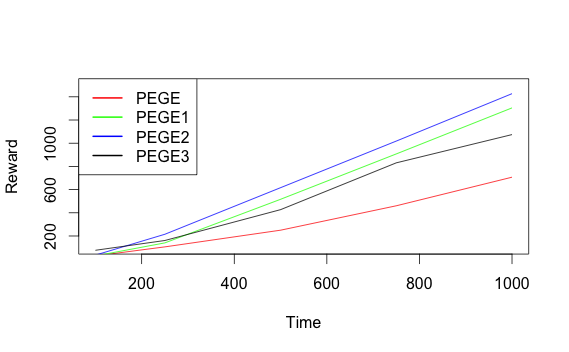
\includegraphics[width=0.50\textwidth,]{algo_compare}
\caption{Comparison of different PEGE algorithms \label{fig: tah0}}
}
\end{figure}




\begin{figure}[htb]
{
\centering
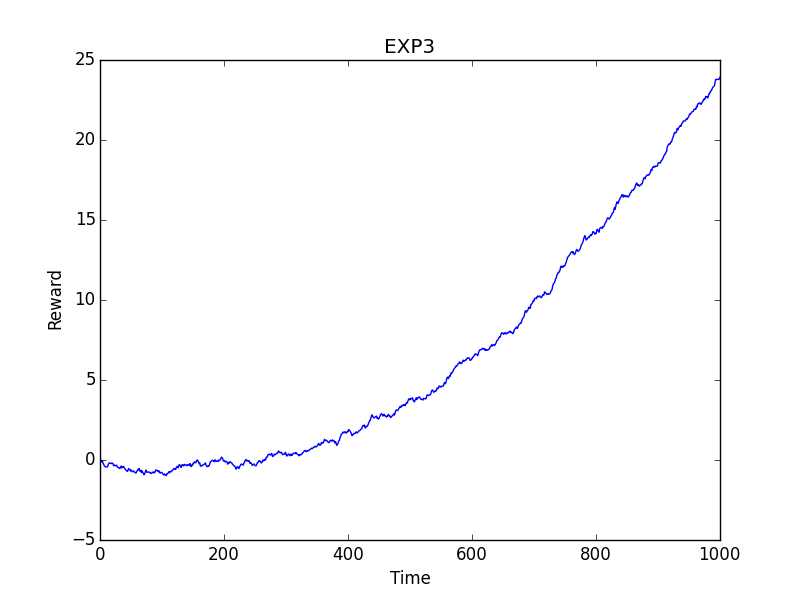
\includegraphics[width=0.50\textwidth]{plot11}
\caption{EXP algorithm. \label{fig: tahi}}
}
\end{figure}

\begin{figure}[htb]
{
\centering
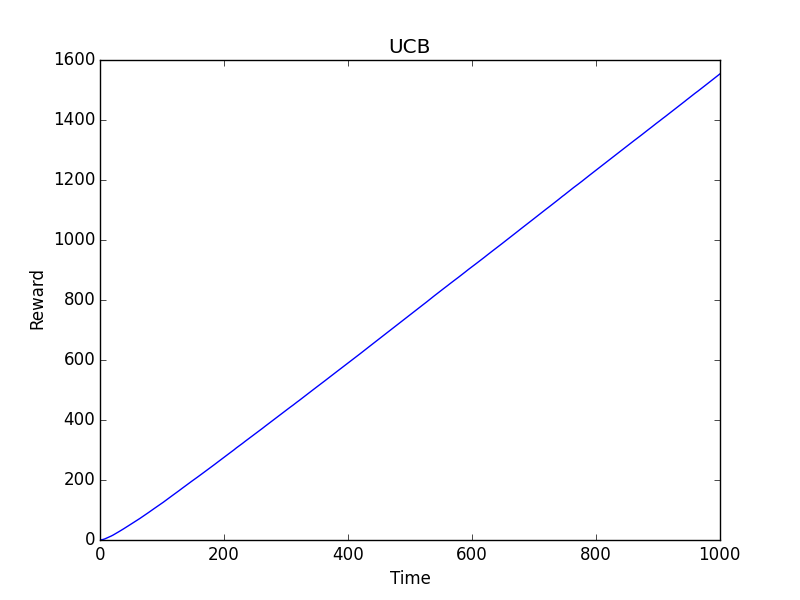
\includegraphics[width=0.50\textwidth]{UCB1}
\caption{UCB algorithm. \label{fig: tah2}}
}
\end{figure}






\section{Conclusion}

In this paper, we studied the linearly parameterized bandits problem, where the reward of each arm linearly depends on a multivariate random variable. In \citet{Paat}, a simple algorithm PEGE is presented, which reaches the optimal Bayes regret bound $O(r\sqrt{T})$. However, the PEGE algorithm does not perform well in practice, since it does the same number of exploitation steps regardless the exploration result. We provided three new PEGE algorithms which balance the number of exploration and exploitation better. We proved that our first heuristic algorithm still has Bayes risk $O(r\sqrt{T})$. Further, we compared our modified algorithms with PEGE as well as UCB and EXP using the Yelp academic dataset. Though UCB performs the best (almost optimal) among these algorithms, it requires a lot of previous information. Our new algorithms which outperformed the PEGE and EXP do not depend on the previous information and can be applied to the ``cold start" problems.


\nocite{langley00}

\bibliography{example_paper}
\bibliographystyle{icml2012}


%\begin{thebibliography}
%[1] Robbins Herbert, \emph{Some aspects of the sequential design of experiments}, Bulletin of the American Mathematical Society 58 (5): 527535
%
%[2] J.C. Gittins, \emph{Bandit Processes and Dynamic Allocation Indices}, Journal of the Royal Statistical Society, Series B (Methodological) 41 (2): 148177
%
%[3] X Zhao, P Frazier, \emph{Exploration vs. Exploitation in the Information Filtering Problem}
%
%[2] Paat Rusmevichientong, John N. Tsitsiklis, \emph{Linearly Parameterized Bandits}
%\end{thebibliography}

\end{document} 



% This document was modified from the file originally made available by
% Pat Langley and Andrea Danyluk for ICML-2K. This version was
% created by Lise Getoor and Tobias Scheffer, it was slightly modified  
% from the 2010 version by Thorsten Joachims & Johannes Fuernkranz, 
% slightly modified from the 2009 version by Kiri Wagstaff and 
% Sam Roweis's 2008 version, which is slightly modified from 
% Prasad Tadepalli's 2007 version which is a lightly 
% changed version of the previous year's version by Andrew Moore, 
% which was in turn edited from those of Kristian Kersting and 
% Codrina Lauth. Alex Smola contributed to the algorithmic style files.  
